\documentclass[12pt]{article}
\usepackage{amsmath}
\usepackage{graphicx,psfrag,epsf}
\usepackage{enumerate}
\usepackage{natbib}
\usepackage{url} % not crucial - just used below for the URL 

%\pdfminorversion=4
% NOTE: To produce blinded version, replace "0" with "1" below.
\newcommand{\blind}{0}

% DON'T change margins - should be 1 inch all around.
\addtolength{\oddsidemargin}{-.5in}%
\addtolength{\evensidemargin}{-.5in}%
\addtolength{\textwidth}{1in}%
\addtolength{\textheight}{1.3in}%
\addtolength{\topmargin}{-.8in}%


\begin{document}

%\bibliographystyle{natbib}

\def\spacingset#1{\renewcommand{\baselinestretch}%
{#1}\small\normalsize} \spacingset{1}


%%%%%%%%%%%%%%%%%%%%%%%%%%%%%%%%%%%%%%%%%%%%%%%%%%%%%%%%%%%%%%%%%%%%%%%%%%%%%%

\if0\blind
{
  \title{\bf Developing Chess With Lua}
  
\begin{figure}
\begin{center}

\includegraphics[width=3in]{luaLogo.png}
\end{center}
\end{figure}
  
  \author{Cameron Wright, Spencer Saunders, Madeline Ross 
    \\Department of Computer Science, Boise State University}
  \maketitle
} \fi

\if1\blind
{
  \bigskip
  \bigskip
  \bigskip
  \begin{center}
    {\LARGE\bf Title}
\end{center}
  \medskip
} \fi



\noindent%
\vfill

\newpage
\spacingset{1.45} % DON'T change the spacing!
%Start of the paper
\section{Introduction}

Lua is a powerful and light language developed in 1993 as a scripting language. It supports procedural programming, object-oriented programming, functional programming, data-driven programming, and data description.  Being chosen as a language for this project had to do with Lua being a language syntactically similar to Python and on the cover it says that Lua is object-oriented.  Simple names like object oriented don't always mean what is the case as is shown when programming chess.

\section{Lua's Syntax}
\subsection{Basic Syntax}
As mentioned in why Lua was chosen as a language for this project, it looks similar to Python with some differences.  In  Figure \ref{fig:LuaSample} it is shown what a simple script would look like, included is functions, variables, and a print statement.  The most similar aspect to Python is where a new line signifies a new step in the program, unlike Java where a ';' signifies the same thing.  The functions are started with keyword 'function' and stop with 'end', this is different from Python which uses the keyword 'def' and knowns when to stop based on tabbing.  Lua does not use tabbing to signify the scope of functions, loops, or conditions, it uses the 'end' keyword.

\begin{figure}
\begin{center}
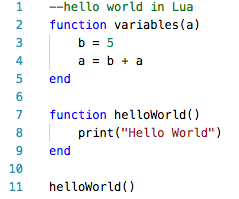
\includegraphics[width=3in]{LuaSample.png}
\end{center}
\caption{\label{fig:LuaSample} Use of white space and variable deceleration in Lua.}
\end{figure}

\section{Naming, Binding, Scoping, Types}
The keyword local is almost always used to define variables and function names as it's good practice.  Variables that are defined as local exist only in the block they're created in.  Lua is a dynamically typed language and doesn't contain any type definitions. Thus, every value carries its own type.  In total, there are eight basic types in Lua which are boolean, number, function, nil, userdata, thread, type, and string.  Variable types are strong and dynamically typed.  No type is needed to declare a variable and after creation it can change between types.  Two different types of objects can not be added together like a String and an int, and if tried the Interpreter will throw and error showing that this language is strongly typed not weak.

\subsection{Defining Class Structure}
Lua was chosen due to a mention of being able to handle object-oriented design principles.  Chess is a game where pieces behave like objects on a board and using object-oriented design patters would prove useful.  Unfortunately Lua's use of classes is much more difficult than it first seems.  Figure \ref{fig:LuaClass} shows the creation of a class, and the amount of extra code needed compared to other languages.  Lua doesn't really have classes, and while to the programmer it is a class to Lua it is an object stored in a metatable.  Back to figure \ref{fig:LuaClass}, the first line of code 'Account = {}' is the creation of the metatable.  Lua's class structure suffers from some major drawbacks from this, and using classes in Lua starts to show some downsides.

The first problem with classes has to do with how they are declared.  The example shown in figure \ref{fig:LuaClass} is not the only way to create a class.  The constructor can be set up multiple ways and even have different names, this adds confusion when looking up how to set up classes on the Internet.  The multiple ways to write classes and lots of boilerplate code starts showing the annoyances of classes in Lua, and there are multiple times throughout this project where a syntactical error was added or incorrectly coding up the class.  Lastly is the subject of inheritance, and how it makes life easier when needing it for generics.  Now Lua at least has inheritance and is something needed with a game like chess where all pieces can relate to a super piece class.  Lua like Python can use classes though Python makes making classes easier, both though are truly scripting languages and both don't support abstract classes.  Not a huge problem but shows the limitations of using classes in a language that is used for scripting.

\begin{figure}
\begin{center}
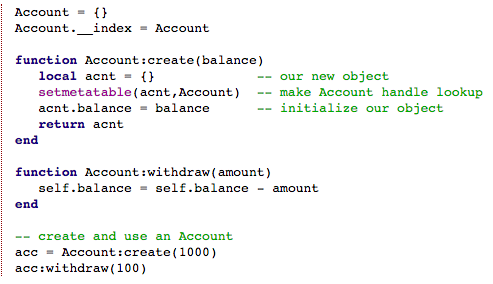
\includegraphics[width=3in]{LuaClass.png}
\end{center}
\caption{\label{fig:LuaClass} Defining a class in Lua.}
\end{figure}


\section{Pros of Lua}
Decent documentation is a plus when working in Lua.  There's a fair number of Wikipedia pages, books, and other various documents put out by the developers and small, but engaged community.  It'd be nice to see additional notes and guides from the developers as the documentation was sufficient but a little barren.  Another is the language has a simplistic, clean syntax that is accessible for beginners and easy to learn.  Lua is has an integrated interpreter that simply requires typing lua in the command line making it convenient to test scripts quickly.  Additionally, the primary data structure in Lua, tables, are versatile and convenient because they're associate and can store values of any type aside from nil. 

\begin{figure}
\begin{center}
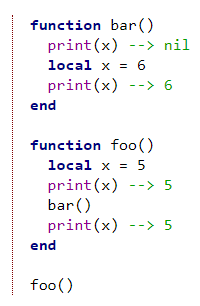
\includegraphics[width=2in]{LuaScope.PNG}
\end{center}
\caption{\label{fig:LuaScope} Figure 3: Scope of a local variable in Lua.}
\end{figure}

\section{Cons of Lua}
One of the major cons of Lua is the lack of built-in language techniques like object-oriented programming without importing a third-party library.  A second major problem with Lua is its lack of error handling.  Error handling support in Lua includes, but is limited to, calling functions pcall and xpcall.  A third problem with Lua is how global scoping is the default of variables and functions.  For instance, if you make a variable called next and then created a function called next in a different module without localizing either, the function will be overwritten. Finally, as mentioned previously, classes in Lua are a hassle as Lua doesn't have the concept of classes and instead has each object define its behavior and shape.

\subsection{Tables, Lua's Solution to Lists and Arrays} \label{tables} 
In Lua, a data structure type called table represents ordinary arrays, queues, sets, and other data structures in a simplified and efficient way.  The table type is implemented and modeled off of associate arrays which allows for indexing with any valid value of Lua including numeric values and strings.  All together Lua is once again like Python where having lists and arrays combine into an amalgamation of the two.  Unlike many other languages that begin indexing at zero, Lua stores its first item at the indexed position of one.  An interesting aspect of tables in Lua is that you can access an indexed position using brackets or a dot. Understanding the difference between bracket and dot indexing is crucial as someone new to Lua may mistakenly use the dot to try and call a function.  Something that happened in this project quite often.  In our Lua Chess implementation, tables played a viable role for functionality as the tables stored the board, all the pieces, all of the valid moves, and other various features.

\section{A Simple Game Called Chess}
Chess is played between two people taking turns moving pieces until someone gets into a position where the king would be checkmated.  Transferring this game into the realm of computers can be easy due to the rules and pieces of the game being few.  For this version of Chess, there still needs to be two players (or you play against yourself) and both will take turns inputing commands.  In this implementation a scanner is used to give a player multiple options about what the want to do, ranging from printing the board, showing moves for a piece, or moving a piece.  When a player puts the other into checkmate the game is finished and either they play again or never again.

\subsection{Using Lua to Create Chess}
Mentioned multiple times throughout this paper, the use of classes and object-oriented design principles was a deciding factor.  In building Chess three layers were used in projecting the game, the board, and the pieces.  A ChessGame is composed of two players who take turns moving pieces.  The board contains a grid of squares and moves the pieces that are currently on the board.  The ChessGame class enforces the rules while the board is only concerned about moving pieces correctly and knowing all the pieces on the board.  Lastly are the pieces which is represented as a Piece superclass and all Pawn, Rook, Knight, Bishop, Queen, and King as subclasses of Piece.  

Plenty of time was spent understanding the class model in Lua and how to have multiple classes inherit or reference each other.  Eventually the use of a library called middleclass was found and used for the creating of classes.  Multiple sources on line that sought a more uniform implementation of classes that got rid of boilerplate code used middleclass.  The use of middleclass in this project reduced class complexity and reduced the number of syntactical errors created by implementing Lua's class system

\section{Conclusion}
Choosing Lua to implement Chess turned out to be a harder-than-expected effort given the easier said than done object oriented claim Lua had. Without this support, the third-party library middleclass was the backbone of the Chess implementation.  Lua certainly has its niche appeal as a scripting language for popular video games like Roblox and Gary's Mod, or the use in embedded systems. However, the group doesn't see themselves using Lua again in the foreseeable future. However, this project was still a valuable and rewarding experience that exposed the group to a lesser-known, under-the-radar language. Throughout the bulk of the project, the various concepts learned in CS354 including scope, types, and semantics made it easier to adjust to and understand the core concepts of Lua.

\end{document}
